%% A simple template for a lab or course report using the Hagenberg setup
%% with the standard LaTeX 'report' class
%% äöüÄÖÜß  <-- keine deutschen Umlaute hier? UTF-faehigen Editor verwenden!

\documentclass[a4paper,twocolumn,english,11pt]{article}		
%\documentclass[a4paper,ngerman,11pt]{article}

\usepackage{hgb}
\usepackage{hgbabbrev}
\usepackage{hgblistings}
\usepackage{hgbbib}
\usepackage{hgbheadings}

\RequirePackage[utf8]{inputenc}		% remove when using lualatex oder xelatex!

\usepackage{lipsum}		% for dummy texts only
\flushbottom

\graphicspath{{images/}}   % where are the images?
\bibliography{literatur}   % requires file 'literatur.bib'


\author{
Peter A.\ Wiseguy\\ 
\texttt{wiseguy@gmail.com}
\and
George Spongehead\\
\texttt{spongehead@gmx.net}}


\title{Reasoning about the unreasonable}
\date{}

%%%----------------------------------------------------------
\begin{document}
%%%----------------------------------------------------------
\maketitle
%%%----------------------------------------------------------

\begin{abstract}
This document shows how to use the standard LaTeX \texttt{article} class in conjunction with the \texttt{hgb.sty}
(Hagenberg) thesis styles. This may be useful, for example, in the case that you wish to publish
part of your thesis as a journal article without major changes.
\end{abstract}


\section{Introduction}

If you wish to write this report in German
you should replace the specification
\begin{verbatim}
\documentclass[a4paper,twocolumn,
                   english]{article}
\end{verbatim}
at the top of this document by
\begin{verbatim}
\documentclass[a4paper,twocolumn,
                   ngerman]{article}
\end{verbatim}
%
Also note that the top sectioning command available in the \texttt{article} class
is \verb!\section{}!, i.e., there are \textbf{no chapters}!
When converting a thesis you thus need to \emph{demote} all chapter commands to
sections, sections to subsections etc.

\subsection{Mathematical elements}

This document is typeset in the typical two-column format required by many
scientific journals. Unfortunately, the narrow text width often creates problems 
with mathematical structures \cite{Voss2014}. 
While smaller equations like
%
\begin{equation}
\bar{\mathbf{M}} =  
\begin{pmatrix}
	A \ast H^{G}_{\sigma}   & C \ast H^{G}_{\sigma} \\
	C \ast H^{G}_{\sigma}   & B \ast H^{G}_{\sigma} 
\end{pmatrix}
=
\begin{pmatrix}
	\bar{A}   & \bar{C} \\
	\bar{C}   & \bar{B} 
\end{pmatrix}
\end{equation}
%
may fit without any modification, larger structures like
the one shown in Equation \ref{wideEquation} need special treatment.
%
\begin{figure*}[t]
\begin{equation}
\begin{split}
\lambda_{1,2} 
&= \frac{\mathrm{tr}(\bar{\mathbf{M}})}{2} \pm \sqrt{\Bigl(\frac{\mathrm{tr}(\bar{\mathbf{M}})}{2}\Bigr)^2 
                      - \mathrm{det}(\bar{\mathbf{M}})}  \\
&= \frac{1}{2} \cdot \left( \bar{A} + \bar{B} \pm \sqrt{\bar{A}^2 - 
		2 \cdot \bar{A} \cdot \bar{B} + \bar{B}^2 + 4 \cdot \bar{C}^2} \right) 
		,
\end{split}
\label{wideEquation}
\end{equation}
\end{figure*}
%
In this case, the equation was wrapped into a
\verb!\begin{figure*}! \ldots \verb!\end{figure*}!
environment, which produces an unnumbered float object that extends
across the full page width.
Additional details can be found in the source text.


\subsection{Graphics and images}

Similarly, the horizontal space available for graphical elements is the width
of a single column. Thus elements inserted with \verb!\includegraphics{..}! 
should use the length \verb!\columnwidth!
for scaling. An example is shown in Fig.~\ref{fig:CocaCola} (see the source text for
details).

\begin{figure}
\centering
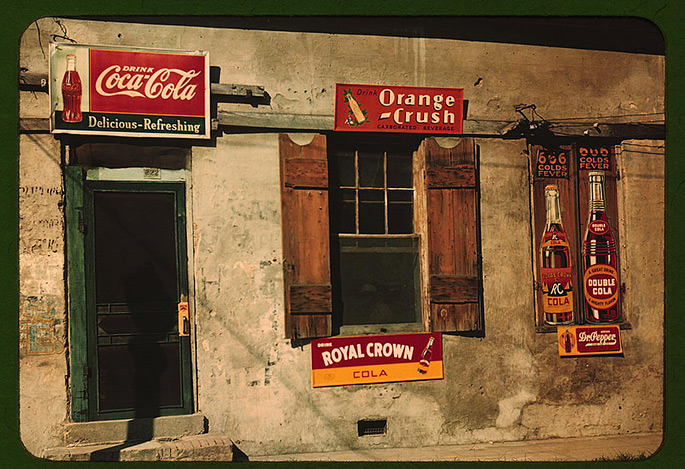
\includegraphics[width=1.0\columnwidth]{cola-public-domain-photo-p}
\caption{Coca-Cola advertisement photographed in 1940 \cite{CocaCola1940}.}
\label{fig:CocaCola}
\end{figure}

An by the way, the \texttt{lipsum} package was used to create the following
dummy texts. 

\subsection{Bibliography}

The use of citations and the compilation of the bibliography works much the same
as in the thesis template. 
The only difference is that \verb!\printbibliography! is used directly at the end
of the document.

\section{Existing techniques}
\lipsum[2-4]


\section{Our radically new approach}
\lipsum[5-7]

\section{Summary and conclusion}
\lipsum[8-9]




%%%----------------------------------------------------------
  
\printbibliography  % alternatively: \MakeBibliography[nosplit]

%%%----------------------------------------------------------

\end{document}
